% REVIEW-READY PILOT MANUSCRIPT, NOT SUBMISSION-READY. Component measurements plus one tiny
% real-model pilot with a negative quality result. Not for submission or publication.
% Figures are read from ../figures relative to this file; regenerate them from public files with
%   .venv/bin/python src/report_results.py --metadata-only
% and compile from the docs/ directory (pdflatex research-draft.tex).
\documentclass[11pt]{article}
\usepackage[margin=1in]{geometry}
\usepackage{graphicx}
\usepackage{hyperref}

\title{Packed Sign Serialization in a Sub-1-Bit Factorized Quantizer:\\
A Component Audit and a Tiny Negative Real-Model Pilot (Review Draft)}
\author{Tim Urista}
\date{Draft of 2026-10-08}

\begin{document}
\maketitle

\begin{center}
\fbox{\parbox{0.9\linewidth}{\textbf{Status.} Review-ready pilot manuscript, not
submission-ready. It reports component measurements of serialization fidelity and storage
accounting, and one bounded local pilot on a real pretrained model with a negative quality
result. It makes no novelty claim, does not replicate any result of the LittleBit papers, and
does not claim that the compressed model is practically useful. The pilot model, Qwen2.5-0.5B, is
smaller than and outside the model table of those papers. Statistical analysis, a validated 4-bit
baseline, a smaller same-family model, task accuracy and end-to-end latency are missing.}}
\end{center}

\begin{abstract}
LittleBit and LittleBit-2 factorize weight matrices into binarized low-rank factors with scale
vectors; the public implementation stores the binary factors packed into 32-bit words. This audit
examines the save and reload round trip of that implementation at commit \texttt{933857e}. In an
exhaustive sweep of 2{,}010 sign patterns through the upstream functions, the unpacker decodes a
$-1$ only at in-word position 0, flipping 21{,}881 signs from $-1$ to $+1$; the packer is correct
and a one-line change restores all cases. In a bounded CPU pilot on Qwen2.5-0.5B, all 168 linear
layers of the transformer blocks were converted at about 0.53 advertised bits per weight and
trained for 16 steps on 2{,}048 tokens. On 1{,}016 held-out WikiText-2 tokens, perplexity was
28.88 for the original model, 82{,}426 for the initialized compressed model and 9{,}736 after
training; the compressed model was worse than the original in all 8 test windows. A corrected
decoder reproduced in-memory logits bitwise after reload on the one 128-token validation window
compared per checkpoint. The pilot is a wiring check, too small for statistical claims, and says
nothing about the methods at their published training budgets.
\end{abstract}

\section{Scope}
The audited code is \url{https://github.com/SamsungLabs/LittleBit} at commit
\texttt{933857ed1443b53fc43a875c2cf64249e3c56f0c}, licensed CC BY-NC 4.0. The methods are due to
Lee, Kim, You and Kim (NeurIPS 2025) and Lee and Kim (ICML 2026). The defect was first observed in
an exploratory run before preregistration; the sweep and layer tests followed a written
preregistration, and the real-model pilot followed a separate preregistration with fixed inputs,
stopping rules and predictions. An official upstream state-dict loading path was executed on a
synthetic single-layer file only; the full-model loader was emulated, not run.

\section{Method}
\subsection{Component audit}
Two evidence tiers are kept separate. \emph{Algorithm audit}: a standard-library mirror of the
upstream arithmetic. \emph{Upstream import}: the unmodified upstream \texttt{binary\_packer},
\texttt{binary\_unpacker} and \texttt{LittleBitLinear}, loaded from the pinned checkout. Two
independent corrected decoders serve as references. The layer benchmark builds upstream layers
from seeded random linear weights, serializes them with the upstream \texttt{state\_dict},
reloads through upstream unpacking, a float32 cast, \texttt{load\_state\_dict(assign=True)} and
binarized inference, and compares outputs with the in-memory layer.

\subsection{Real-model pilot}
Model: Qwen/Qwen2.5-0.5B, revision \texttt{060db649}, Apache-2.0. Data: WikiText-2 raw, revision
\texttt{b08601e0}; train, validation and test split prefixes tokenized separately with the native
tokenizer, cut into contiguous non-overlapping 128-token windows (16 train, 4 validation, 8
test), each identified by the SHA-256 of its token ids. The first token of each window is not
scored.

Every \texttt{nn.Linear} in the 24 transformer blocks (168 modules, 357{,}826{,}560 weights) was
converted to the upstream \texttt{LittleBitLinear} with \texttt{eff\_bit} 0.55, residual path,
SVD initialization and SmoothSign. Embeddings, the tied output head, norms and biases were
frozen. The objective was next-token cross entropy plus KL(teacher $\|$ student), averaged over
positions, weight 1.0 each, with the frozen original model as teacher. AdamW, learning rate
$4\times10^{-5}$, cosine decay, gradient clip 1.0, batch 1, 16 steps, each train window used once:
2{,}048 input tokens and 2{,}032 supervised targets. CPU, float32, 2 threads, seed 42, one run.
Declared departures from upstream training are listed in the preregistration (float32 on CPU,
token-mean KL, added cross entropy, no intermediate hidden-state loss, frozen norms and biases).

Initialized and trained students were each saved (packed signs from the upstream packer, float32
scales, frozen tensors in a separate file), reloaded with a corrected decoder, and scored on the 8
test windows. The same trained weights were also reloaded in memory with the shipped unpacker and
scored as a separately labeled defect variant. Identity was checked on a validation window by
comparing in-memory and reloaded logits and loss.

\section{Results}
\subsection{Exhaustive unpack sweep}
The unpack expression \texttt{(word << k) \& 1} clears bit 0 for every $k \ge 1$. A row decodes
exactly if and only if all of its $-1$ entries lie at columns $j$ with $j \bmod 32 = 0$; this rule
predicted all 2{,}010 cases.

\begin{center}
\begin{tabular}{lrrrrrrr}
\hline
width & 1 & 7 & 8 & 31 & 32 & 33 & 64 \\
\hline
byte rows exact (of 256) & 256 & 4 & 2 & 1 & 1 & 1 & 1 \\
sign errors & 0 & 786 & 917 & 3930 & 4062 & 4062 & 8124 \\
\hline
\end{tabular}
\end{center}

\subsection{Layer round trip and patch}
Across 72 seeded configurations the upstream decoder kept 0.514 to 0.553 of the signs and changed
all 72 outputs; a corrected decoder kept all signs and gave bitwise equal outputs in all 36
float32 configurations. Applied in memory to the unmodified source, the one-line change from
\texttt{<<} to \texttt{>>} decoded 2{,}010 of 2{,}010 sweep cases exactly (296 without it) and
restored every factor, including residual factors, in five upstream layers. On a synthetic
single-layer file loaded through the official state-dict path, sign agreement was 0.531 to 0.586
with the shipped decoder and 1.0, with bitwise equal output, with the corrected decoder.

\subsection{Real-model pilot: held-out quality}
Table~\ref{tab:ppl} and Figures~\ref{fig:ppl} and~\ref{fig:paired} report token-weighted
perplexity and per-window mean negative log-likelihood (NLL) on the same 1{,}016 test tokens.

\begin{table}[h]
\centering
\begin{tabular}{lrrr}
\hline
condition & perplexity & mean NLL & windows worse than original \\
\hline
original & 28.8816 & 3.3632 & reference \\
initialized, no QAT & 82{,}426.3372 & 11.3197 & 8 of 8 \\
16-step QAT & 9{,}735.6350 & 9.1835 & 8 of 8 \\
same QAT weights, defective decoder & 13{,}558{,}558.4902 & 16.4225 & 8 of 8 \\
\hline
\end{tabular}
\caption{Held-out perplexity on 8 WikiText-2 test windows (1{,}016 scored tokens). The last row is
a decoder defect variant, not a quality result.}
\label{tab:ppl}
\end{table}

Per-window NLL increases over the original were 7.23 to 8.71 nats for the initialized student and
5.13 to 6.51 nats after training. Training lowered NLL relative to initialization in all 8 windows
(by 1.81 to 2.52 nats), leaving perplexity about 337 times the original (about 2{,}854 times
before training). These are descriptive figures: the 8 windows are contiguous segments of one
test prefix, not independent samples, and there is a single seed and run, so no intervals or
tests are reported. The preregistered predictions that the initialized student would be at least
10 times and the trained student at least 5 times worse than the original both held.

\begin{figure}[h]
\centering
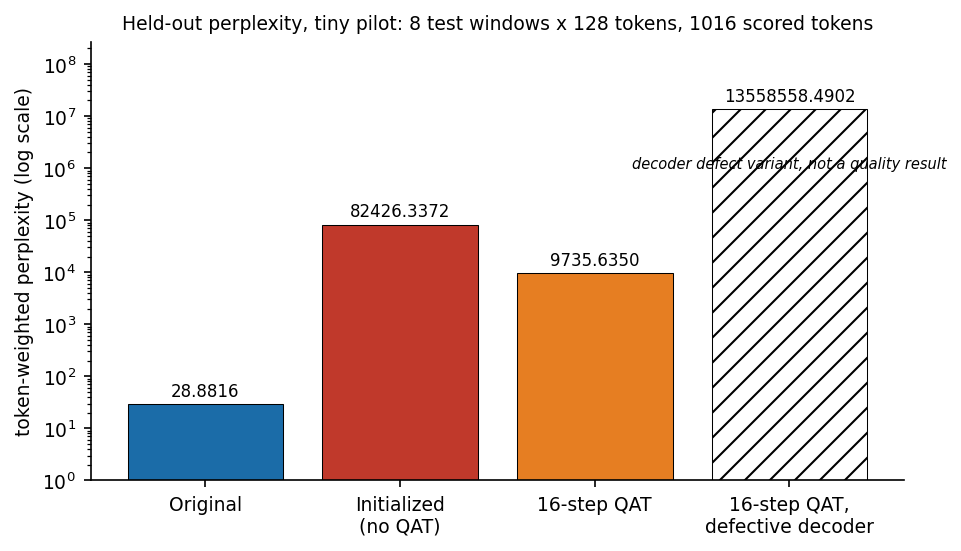
\includegraphics[width=0.75\linewidth]{../figures/heldout_ppl_log.png}
\caption{Token-weighted held-out perplexity, log scale, tiny pilot of 1{,}016 scored tokens. The
hatched bar uses the defective upstream decoder on the same trained weights.}
\label{fig:ppl}
\end{figure}

\begin{figure}[h]
\centering
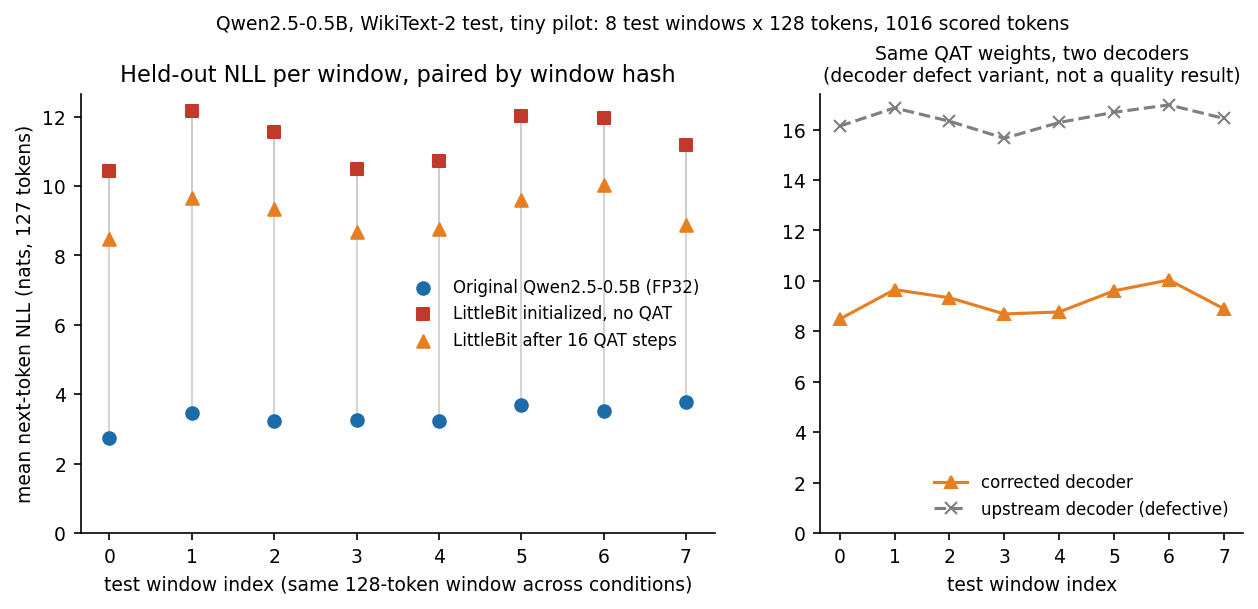
\includegraphics[width=\linewidth]{../figures/paired_window_nll.png}
\caption{Per-window held-out NLL, paired by window hash. Left: original, initialized and trained
students. Right: the same trained weights under the corrected and the defective decoder.}
\label{fig:paired}
\end{figure}

\subsection{Training trace and reload identity}
Cross entropy and KL per step are shown in Figure~\ref{fig:train}. Cross entropy rose from 13.41
at step 0 to 26.58 at step 1 and ended at 9.45; KL went from 9.42 to 23.62 and ended at 6.03. With
the corrected decoder, all 171{,}294{,}720 signs agreed and logits and loss were bitwise identical
between the in-memory and reloaded students, for both the initialized and the trained checkpoint,
on CPU in float32. Logits and loss were compared on one 128-token validation window per
checkpoint only. The teacher parameter fingerprint was unchanged by training. Training flipped
360{,}930 signs (0.21\%).

\begin{figure}[h]
\centering
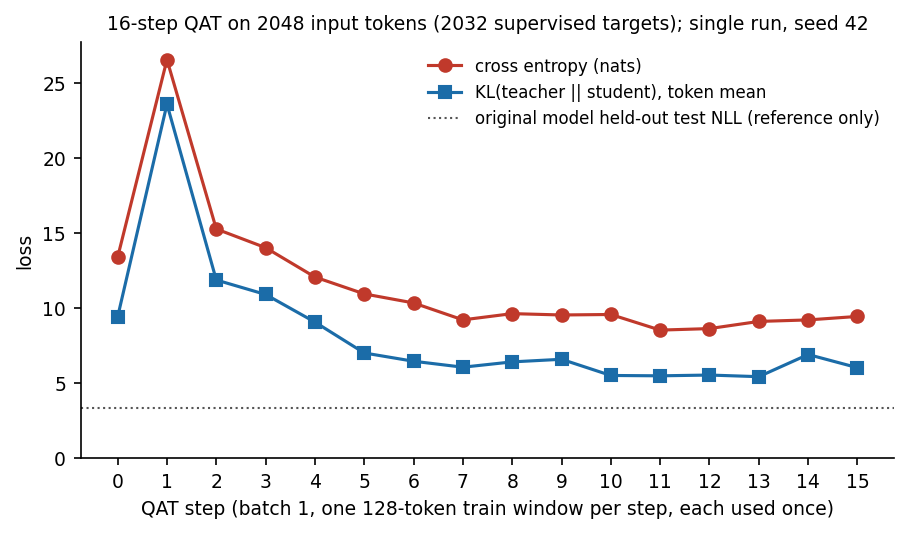
\includegraphics[width=0.75\linewidth]{../figures/train_ce_kl.png}
\caption{Cross entropy and token-mean KL per QAT step, one 128-token window per step, single run.}
\label{fig:train}
\end{figure}

\subsection{Storage}
Disk and resident bytes are reported separately because they use different data types;
tokenizer and configuration files (15{,}879{,}995 bytes) are excluded throughout
(Figure~\ref{fig:bytes}). For the converted block linears, the upstream formula gives 0.52955 bits
per weight, packed signs alone 0.4967, and the actual compressed checkpoint file with float32
scales 0.6094. On disk, the original BF16 weight file is 988{,}097{,}824 bytes; the pilot stores
a frozen BF16 base of 272{,}426{,}320 bytes, of which 272{,}269{,}312 are the embedding table,
plus 27{,}257{,}280 bytes of compressed layers. Resident unique tensor storage in float32 is
1{,}976{,}131{,}200 bytes for the original model and 1{,}234{,}703{,}616 bytes for the student, of
which 544{,}538{,}624 bytes in each are the embedding table and 689{,}878{,}656 bytes are
LittleBit factors, scales and buffers held as float32. The 128-token float32 KV cache is 3~MiB in
both cases.

\begin{figure}[h]
\centering
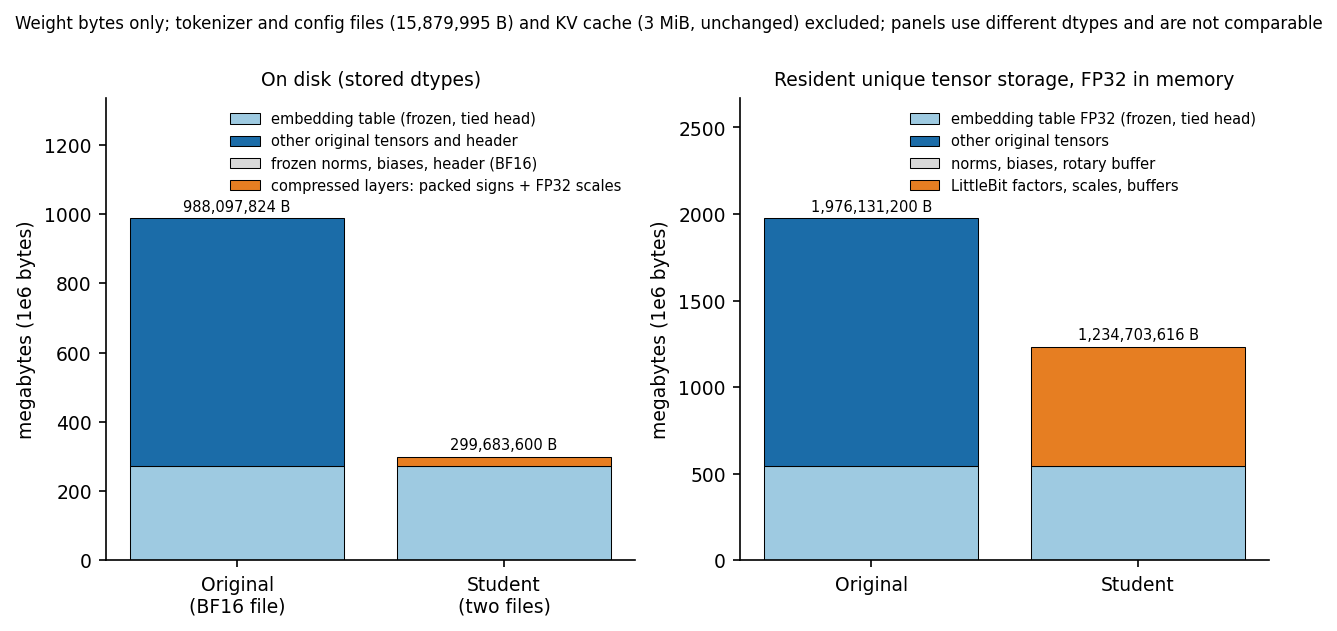
\includegraphics[width=\linewidth]{../figures/weight_bytes.png}
\caption{Weight bytes on disk (stored dtypes, left) and resident unique tensor storage in float32
(right), with the frozen embedding table shown separately. The panels are not comparable with
each other.}
\label{fig:bytes}
\end{figure}

\subsection{Resources}
The training stage took 82.36~s of wall clock, including 8.98~s of conversion; steps took 2.53 to
5.32~s. The operating system reported a peak resident set of 6.53~GiB, above the preregistered
6~GiB guard threshold. The guard samples memory at checkpoints (highest sampled value 5.34~GiB)
and is not a hard cap, so the run was not stopped; the preregistered memory prediction (4.5 to
6.0~GiB) failed. No further training is planned.

\section{Discussion}
\paragraph{Significance.} The serialization defect is a concrete, reproducible deployment issue
with a one-line fix: checkpoints saved with this code lose most of their $-1$ signs when loaded
with the shipped unpacker, and on the pilot model this moves held-out perplexity from 9{,}736 to
over 13 million on the same weights. The pilot quality result is negative: at about 0.53
advertised bits per weight, a 16-step budget on a 0.5B model leaves perplexity about 337 times
the original. Because model, budget, precision and hardware all differ from the published
settings, this is not evidence for or against the reported LittleBit results.

\paragraph{Application.} The transferable parts are procedural: exhaustive sign sweeps for
packed formats; separate initialized and trained results on frozen, hashed, paired windows; a
bitwise reload identity check before any quality or speed number; and byte accounting that keeps
disk, resident and KV memory apart and states the dtype of each.

\section{Limitations}
One model outside the papers' model table, one seed, one run, 16 steps, 2{,}048 training tokens
and 1{,}016 scored tokens; no statistical analysis. No validated 4-bit baseline, no smaller
same-family model, no task accuracy, no end-to-end latency or throughput. Float32 CPU training
with declared departures from the upstream recipe. Full-model loading emulated. The memory guard
is sampled rather than enforced. Component layers in the sweep and layer tests use random weights.

\section*{Data and code availability}
Code, raw stage outputs, preregistrations, figures and a summary are released as version v0.1.0
at \url{https://github.com/timurista/littlebit-deployment-audit/releases/tag/v0.1.0}. The release
carries a build manifest recording the exact commit and SHA-256 checksums of its files. No DOI has
been assigned. Figures and summary are regenerated from
tracked public files with \texttt{python src/report_results.py --metadata-only}, without running
a model; that replay does not validate the pilot checkpoints, which were validated privately on
the author's host and are not redistributed. Model weights, derived checkpoints, dataset files and
the upstream checkout are not redistributed.

\section*{Licensing}
No license is granted for the original code of this audit: all rights are reserved by the author,
and a license is proposed but not enacted (\texttt{LICENSE\_PROPOSAL.md}). Portions that adapt or
quote upstream code remain under CC BY-NC 4.0, with attribution and NonCommercial obligations.
Upstream code is CC BY-NC 4.0; Qwen2.5-0.5B is Apache-2.0; WikiText-2 is distributed under CC
BY-SA terms. No license agreement was accepted and no cloud resources were used.

\section*{AI assistance}
The code, tests and text of this draft were written with an AI coding assistant (Claude,
Anthropic). The experiments were executed by an automated AI coding workflow on the author's Mac,
not run by hand; the author's review of the outputs is pending. All reported numbers are taken
from recorded output files.

\section*{Attribution}
LittleBit and LittleBit-2 by B.~Lee, D.~Kim, Y.~You and Y.~Kim. Code under CC BY-NC 4.0. This
audit is not affiliated with or endorsed by the authors or Samsung.

\end{document}
